\begin{filecontents*}{example.eps}
%!PS-Adobe-3.0 EPSF-3.0
%%BoundingBox: 19 19 221 221
%%CreationDate: Mon Sep 29 1997
%%Creator: programmed by hand (JK)
%%EndComments
gsave
newpath
  20 20 moveto
  20 220 lineto
  220 220 lineto
  220 20 lineto
closepath
2 setlinewidth
gsave
  .4 setgray fill
grestore
stroke
grestore
\end{filecontents*}
%
\RequirePackage{fix-cm}
%
%\documentclass{svjour3}                     % onecolumn (standard format)
%\documentclass[smallcondensed]{svjour3}     % onecolumn (ditto)
%\documentclass[smallextended]{svjour3}       % onecolumn (second format)
\documentclass[twocolumn]{svjour3}          % twocolumn
%
\smartqed  % flush right qed marks, e.g. at end of proof
%
\usepackage{graphicx}


\usepackage{amsmath}
\usepackage{amssymb}
\usepackage{mathtools}
\usepackage{algorithm}
\usepackage{algorithmic}
%
\usepackage{mathptmx}      % use Times fonts if available on your TeX system
%
% insert here the call for the packages your document requires
%\usepackage{latexsym}
% etc.
%
% please place your own definitions here and don't use \def but
% \newcommand{}{}
%
% Insert the name of "your journal" with
% \journalname{myjournal}
%

\newcommand{\tit}[1]{\textit{#1}}
\renewcommand{\rm}[1]{\textrm{#1}}
\newcommand{\bb}[1]{\mathbb{#1}}
\renewcommand{\cal}[1]{\mathcal{#1}}
\newcommand{\te}[1]{\text{#1}}
\newcommand{\ep}{\varepsilon}
\renewcommand{\bf}[1]{\mathbf{#1}}

\begin{document}

\title{Insert your title here%\thanks{Grants or other notes
%about the article that should go on the front page should be
%placed here. General acknowledgments should be placed at the end of the article.}
}
\subtitle{Do you have a subtitle?\\ If so, write it here}

%\titlerunning{Short form of title}        % if too long for running head

\author{First Author         \and
        Second Author %etc.
}

%\authorrunning{Short form of author list} % if too long for running head

\institute{F. Author \at
              first address \\
              Tel.: +123-45-678910\\
              Fax: +123-45-678910\\
              \email{fauthor@example.com}           %  \\
%             \emph{Present address:} of F. Author  %  if needed
           \and
           S. Author \at
              second address
}

\date{Received: date / Accepted: date}
% The correct dates will be entered by the editor


\maketitle

\begin{abstract}
Insert your abstract here. Include keywords, PACS and mathematical
subject classification numbers as needed.
\keywords{First keyword \and Second keyword \and More}
% \PACS{PACS code1 \and PACS code2 \and more}
\subclass{MSC code1 \and MSC code2 \and more}
\end{abstract}

\section{Introduction}
\label{intro}
Your text comes here. Separate text sections with

\section{Preliminaries}

In this section, we introduce the Grad-Shafranov equation and describe the
neural operator architectures used in this work.

\subsection{Grad-Shafranov Equation}
The Grad-Shafranov equation describes the steady-state plasma equilibrium within
the framework of ideal magnetohydrodynamics (MHD), under the assumption that
the plasma is axisymmetric.

Let $(R, \phi, Z)$ be a cylindrical coordinate system with $R > 0$.
We define $\Omega = (0, R_{max})\times (-Z_{max}, Z_{max})$ as a 2D computational domain 
in the coordinates $(R, Z)$. We also define the plasma domain $\Omega_p\subset \Omega$ 
as the region occupied by the plasma.
The corresponding plasma boundary is denoted by $\partial \Omega_p$.
In many cases, determining or controlling the plasma domain is a central issue
in plasma equilibrium problems.
% We will discuss more about the plasma boundary in the Section~\ref{sec:2.1.2} and 
% Figure~\ref{fig:boundary}.

The Grad-Shafranov equation reads
\begin{align}\label{eq:1}
  \Delta^* \psi(R, Z) = -\mu_0 R J_\phi(R, Z; \psi), \quad (R, Z) \in \Omega,
\end{align}
where $\psi = \psi(R, Z)$ is the axisymmetric poloidal flux function,
$\mu_0$ is the vacuum permeability, and $J_\phi$ is the toroidal current density.
The operator $\Delta^*$ is an elliptic operator with cylindrical coordinates, defined by
$\Delta^* = \frac{\partial^2}{\partial R^2} - \frac{1}{R}\frac{\partial}{\partial R} + 
\frac{\partial^2}{\partial Z^2}$.
To close the equation, we have to determine the toroidal current density $J_\phi$ and the boundary condition.

\subsubsection{Modeling of the toroidal current density $J_\phi$}

The toroidal current density $J_\phi$ depends not only on nonlinear functions of $\psi$ and 
on the plasma boundary, but also on external environments, such as currents in the active coils.
To be more precise, $J_\phi$ can be decomposed into two parts, 
\begin{align}
  J_\phi(R, Z; \psi) = J_{\text{p}, \phi}(R, Z; \psi) + J_{\text{m}}(R, Z),
\end{align}
where $J_{\text{p}, \phi}$ is the plasma current density and 
$J_{\te{m}}$ is the current density due to the external coils. 
For simplicity, we treat $J_\te{m}$ as fixed; in general, however,
$J_\te{m}$ is a main control variable for the plasma equilibrium problems.

The plasma current density $J_{\text{p}, \phi}$ is composed of the pressure $p = p(\psi)$ and the 
toroidal magnetic field function $F = F(\psi)$;
\begin{align}\label{eq:3}
  J_{\te{p}, \phi}(R, Z; \psi) = \begin{cases}
  \begin{aligned}
  & R p'(\psi)(R, Z) + \\
  & \quad \frac{1}{R} \left(F(\psi)F'(\psi)\right)(R, Z)
  \end{aligned} &  (R, Z) \in \Omega_p \\
  0 & (R, Z) \in \Omega \setminus \Omega_p
\end{cases}, \end{align}
where $p'(\psi)$ and $F'(\psi)$ are the derivatives of $p$ and $F$ with respect to $\psi$, respectively. 
Thus, the plasma current density is affected by the plasma boundary. 
In the next subsection, we will discuss how to determine the plasma boundary.

Several models have been proposed for $p'(\psi)$ and $F'(\psi)$. 
Here, we adopt the Lao-type profile parametrization \cite{lao} for the plasma current density.
\begin{align*}
  J_{\phi, \rm{pl}}(R, Z; \psi) =
  \lambda &\left[\beta_0 \frac{R}{R_{\rm{geo}}}\tilde{j}_p(\psi, \psi_a, \psi_b) + \right. \\
  & \ \left. (1-\beta_0) \frac{R_{\rm{geo}}}{R}\tilde{j}_F(\psi, \psi_a, \psi_b)\right]
  \bf{1}_{\Omega_{\rm{p}}}(R, Z),
\end{align*}
where $R_{\te{geo}}$ is the major radius of the plasma;
$\lambda$ and $\beta_0$ are the normalization constants, with details of the 
normalization given in Appendix~\ref{sec:normalization}.
Here $\tilde{j}_p$ and $\tilde{j}_F$ are the normalized pressure and 
toroidal magnetic field profiles: 
\begin{align*}
  \tilde{j}_p(\psi, \psi_a, \psi_b) &= (1 - \psi_s^{\alpha_m})^{\alpha_n} \\
  \tilde{j}_F(\psi, \psi_a, \psi_b) &= (1 - \psi_s^{\beta_m})^{\beta_n} \\
  \psi_s &= \frac{\psi - \psi_a}{\psi_b - \psi_a}, \\
\end{align*}
The parameters $\alpha_m, \alpha_n, \beta_m, \beta_n$ determine  
the shapes of the pressure and toroidal field profiles,
and the quantities $\psi_a$ and $\psi_b$ are the poloidal-flux values
at the plasma magnetic axis and at the plasma boundary, respectively.
We discuss these quantities further in the next subsection.

For later use, we decompose $\psi = \psi_\text{p} + \psi_\text{m}$,
taking advantage of the linearity of  the left-hand side of the Grad-Shafranov equation,
where $\psi_\te{p}$ satisfies
\[ \Delta^* \psi_\te{p}(R, Z) = -\mu_0 R J_{\text{p}, \phi}(R, Z; \psi), \]
and $\psi_\te{m}$ satisfies
\[ \Delta^* \psi_\te{m}(R, Z) = -\mu_0 R J_{\text{m}}(R, Z). \]
Note that $J_{\text{p}, \phi}$ is a function of $\psi$, not $\psi_\te{p}$.

Given $J_\phi$, we can obtain the value of $\psi$ at the computational boundary $\partial \Omega$.
Let $\psi_{\te{bdry}}: \partial \Omega \to \bb{R}$ denote the boundary value of $\psi$ on $\partial \Omega$.

\begin{align}\label{eq:4}
  \psi_{\te{bdry}}(R, Z) = \iint_\Omega G(R, Z; R', Z') J_\phi(R', Z'; \psi) dR' dZ',
\end{align} 
where $(R, Z) \in \partial \Omega$ and $G$ is the Green's function for the operator $\Delta^*$;
\begin{align*} G(R, Z; R', Z') &= \frac{\mu_0}{2 \pi} \frac{\sqrt{R R'}}{k} \left[
  (2 - k^2) K(k) - 2E(k) 
\right], \\ k^2 &= \frac{4 R R'}{(R + R')^2 + (Z - Z')^2} \end{align*}
and $K$ and $E$ are the complete elliptic integrals of the first and second kind, respectively.

\subsubsection{Determination of the plasma boundary} \label{sec:2.1.2}
In the free-boundary problem, the plasma boundary is not known a priori, and
hence it is determined by the solution $\psi$ itself.
More precisely, given the plasma flux $\psi$ and the geometry of the tokamak,
the plasma boundary value $\psi_b$ is determined by the following procedure.
Assume the total plasma current 
\[ I_p = \int_{\Omega_p} J_{\text{p}, \phi}(R, Z; \psi) \, dR \, dZ > 0. \]
Then the poloidal flux $\psi$ typically attains a minimum at the plasma magnetic axis, and increases toward the plasma boundary.
If a saddle point of $\psi$, called the X-point, exists inside the tokamak structure, 
the plasma boundary value is determined at the value of $\psi$ at the X-point.  
In this case, we say that the plasma is diverted. 
The minimum value of $\psi$ is attained at the plasma magnetic axis, denoted by $\psi_a$
as mentioned above.
Therefore, we identify candidate critical points where $|\nabla \psi|$ is close to zero,
and we then compute the Hessian matrix of $\psi$ at each candidate point to classify it as 
either the magnetic axis or the X-point.
Then the value of $\psi$ at the X-point is the plasma boundary value $\psi_b$, and 
the value of $\psi$ at the magnetic axis is $\psi_a$. 
For $I_p < 0$, the roles of local minimum and maximum are reversed; 
in particular, the plasma magnetic axis corresponds to the local maximum of $\psi$. 

On the other hand, because the domain $\Omega$ is bounded, in some cases 
all saddle points of $\psi$ may lie outside the tokamak structure, and hence the plasma boundary is
determined by the limiter, which is a material structure of the tokamak.
In this case, the plasma boundary value $\psi_b$ is determined by the largest/smallest value of $\psi$ on the limiter-facing surface when $I_p > 0$/$I_p < 0$. In this case, the plasma is limited.

Finally, the plasma boundary is the level set of $\psi_b$;
\[ \partial \Omega_p = \{(R, Z) \in \Omega: \psi(R, Z) = \psi_b\}. \]
See Figure~\ref{fig:boundary} for examples of the plasma boundary.

Given the plasma boundary, the plasma current density $J_{\text{p}, \phi}$ 
and the correspoinding boundary value of $\psi_{\te{bdry}}$ 
are obtained by \eqref{eq:3} and \eqref{eq:4}, respectively.


\subsection{Numerical methods for solving the Grad-Shafranov equation}

Because $J_\phi$ depends on $\psi$, the equation is nonlinear. 
Thus, the numerical solution of the Grad-Shafranov equation is obtained
by iteratively solving the equation with an updated $J_\phi$ until convergence.

In particular, we start with an initial guess $\psi^{(0)}$.
Given this initial guess, suppose that the previous iterate $\psi^{(n-1)}$
is available for $n \geq 1$.
Then we first determine the plasma domain $\Omega_p^{(n-1)}$ from $\psi^{(n-1)}$, 
and we compute the toroidal current density $J_\phi(\cdot ; \psi^{(n-1)})$ 
on the computational domain $\Omega$ and $\psi_{\te{bdry}}^{(n-1)}$ at $\partial \Omega$ 
with the plasma domain $\Omega_p^{(n-1)}$ and the previous iterate $\psi^{(n-1)}$.
Because the plasma current density is recomputed from the updated
current density, note that the newly obtained 
$\psi_{\te{bdry}}^{(n-1)}$ need not coincide with the $\psi^{(n-1)}$ on the boundary $\partial \Omega$. 
Then we can obtain the solution $\psi^{(n)}$ by solving the one-step 
Grad-Shafranov equation;
\begin{align}\label{eq:5}
  \left\{
  \begin{aligned}
    \Delta^* \psi^{(n)}(R, Z) &= -\mu_0 R J_\phi(R, Z; \psi^{(n-1)}), \quad (R, Z) \in \Omega, \\
    \psi^{(n)}(R, Z) &= \psi_{\text{bdry}}^{(n-1)}(R, Z; \psi^{(n-1)}), \quad (R, Z) \in \partial \Omega,
  \end{aligned}
  \right.
\end{align}
and we repeat the above procedure until convergence. 
For later use, we formulate it in the operator form. 
Let $\cal{F}$ be the one-step solution operator, defined by
\[ \cal{F}[\psi^{(n-1)}] = \psi^{(n)}, \]
where $\psi^{(n)}$ is the solution of the one-step Grad-Shafranov equation \eqref{eq:5} with 
$J_\phi(\cdot ; \psi^{(n-1)})$ and $\psi_{\text{bdry}}^{(n-1)}$.
Then its fixed point is the exact solution for the Grad-Shafranov equation.
% Equivalently, we consider the residual operator $\cal{R}$ defined as 
% $\cal{R}[\psi] = \psi - \cal{F}[\psi]$, and the solution
% of the Grad-Shafranov equation is the root of $\cal{R}.$

Several numerical methods can be used to solve the one-step Grad-Shafranov equation.
Since in most cases the computational domain $\Omega$ is the extended area of the 
tokamak structure, its geometry is often simple.
Also the differential operator $\Delta^*$ is linear.
Thus standard finite difference methods with central differences are widely used.
However, in general $\cal{F}$ is not a contraction, and several studies have reported that
there are multiple solutions for the Grad-Shafranov equation,
and hence the convergence of the above procedure is not guaranteed.
% For example, with 

Alternatively, when $\psi^{(n)}$ is close to the solution, 
the Jacobian-free Newton-Krylov method can be used to solve the one-step Grad-Shafranov equation.
Because the boundary computation for the plasma is included to compute $\cal{F}$,
it is difficult to compute its Jacobian matrix with respect to $\psi$.
Meanwhile, the standard Newton Krylov method only requires the matrix-vector product of the Jacobian matrix, not the Jacobian matrix itself.
Therefore, we approximate the Jacobian matrix $\cal{J}[\psi](\Delta \psi)$ 
by the finite difference method;
\[ \cal{J}[\psi](\Delta \psi) \approx 
\frac{\cal{F}[\psi + \epsilon \Delta \psi] - \cal{F}[\psi]}{\epsilon} \]
for $\epsilon > 0$ a small constant.
We perform Arnoldi iteration with this formulation to compute the Krylov subspace,
and solve the least squares problem to obtain the update direction $\Delta \psi$.
(Details of the Jacobian-free Newton-Krylov method are provided in Appendix~\ref{sec:JFNK}.)

Our method is designed to serve as a neural surrogate 
for the numerical solver, to replace the operator $\cal{F}$ so the overall 
procedure can be accelerated.
% , as we will describe in the next section.
In this work, our neural network assisted approach is combined to the 
freegsnke solver \cite{freegsnke},
which uses both a finite difference method and a Jacobian-free Newton-Krylov 
method to solve the one-step Grad-Shafranov equation. 

% 내일 neural operator background & method 채우기


\subsection{Physics-Informed Neural Operators}

Neural operators (NOs) \cite{NOs} are a class of neural networks designed to learn mappings between function spaces.
Let $\cal{X}$ and $\cal{Y}$ be Banach spaces of functions defined on the bounded domain. 
Our task is to approximate an operator 
\[ \cal{N}: \cal{X} \to \cal{Y}, \]
using a neural network $\cal{N}_\theta$.
In general, to train the neural operator, one typically uses a dataset 
$\{(v_i, u_i = \cal{N}(v_i)) \}_{i=1}^N$ where $v_i \in \cal{X}$ and $u_i \in \cal{Y}$ 
are the input and output functions, respectively.
Then the neural operator $\cal{N}_\theta$ is trained to minimize the loss function 
\[ L(\theta) = \frac{1}{N}\sum_{i=1}^N \|\cal{N}_\theta(v_i) - u_i \|^2 \]
where the norm is defined on the function space $\cal{Y}$, and in practice, 
it is approximated by the discrete $L^2$ norm on the grid points.

Physics-informed neural operators (PINOs) \cite{PINOs} combine 
the neural operator framework with a physics-informed loss function, 
which allows them to learn without relying on solution data. 
Consider a general parametrized elliptic PDE with the form 
\begin{align}\label{eq:6}
  \begin{cases}
    \cal{L}[u](x) = f(x;v), & x \in \Omega, \\
    \cal{B}[u](x) = g(x;v), & x \in \partial \Omega.
  \end{cases}
\end{align}
Here, $v \in \cal{X}$ affects the source term $f$ and the boundary condition $g$, and 
$u \in \cal{Y}$ is the solution of the PDE, $\cal{L}$ is the differential operator, and
$\cal{B}$ is the boundary operator.
The goal is to learn the operator $\cal{N}: \cal{X} \to \cal{Y}$ which maps
$v$ to $u$, with the input data $\{ v_i \}_{i=1}^{N_\te{data}}$ and the governing PDE, 
without access to the corresponding solutions $\{u_i\}_{i=1}^N$.

The physics-informed loss function can be written as
\begin{align}\label{eq:7}
  \begin{aligned}
    L(\theta) &= L_\te{r}(\theta) + L_\te{b}(\theta) \\
    L_\te{r}(\theta) &= \frac{1}{N}\sum_{i=1}^N \int_\Omega |\cal{L}[\cal{N}_\theta(v_i)](x) - f(x;v_i)|^2 dx, \\
    L_\te{b}(\theta) &= \frac{1}{N}\sum_{i=1}^N \int_{\partial \Omega} |\cal{B}[\cal{N}_\theta(v_i)](x) - g(x;v_i)|^2 dx.
  \end{aligned}
\end{align}
In our case, for a given previous iterate $\psi^{(n-1)}\in \cal{X} \subset H^2(\Omega)$, 
the one-step Grad-Shafranov solution belongs to 
$\cal{Y}_{\psi^{(n-1)}} = \{ u \in H^2(\Omega) : 
u|_{\partial \Omega} = \psi_{\te{bdry}}|_{\partial \Omega} \}$,
where $H^2(\te{int }\Omega)$ denotes the Sobolev space of functions with 
square-integrable second derivatives. 
Also for $\psi^{(n-1)} \in \cal{X}$,
\begin{align*}
  \cal{L} &= \Delta^*, \quad \cal{B}[\psi^{(n-1)}] = \psi^{(n-1)}_{\te{bdry}},  \\
  f(R, Z; \psi^{(n-1)}) &= -\mu_0 R J_\phi (R, Z; \psi^{(n-1)}),  \\
  g(R, Z; \psi^{(n-1)}) &= \psi_{\te{bdry}}(R, Z; \psi^{(n-1)}).
\end{align*} 

In this work, we use a combination of physics-informed DeepONet 
and the physics-informed neural transformer operator,
to predict the solution of the one-step Grad-Shafranov equation.
We train these two models using the physics-informed formulation described above. 
In the next two subsections, the architectures of the two models are described in detail.

\subsubsection{Physics-Informed DeepONet}

DeepONet \cite{deeponet} is one of the most widely used neural operators, 
and it is based on the universal approximation theorem for operators. 
Its structure is composed of two sub-networks, called the branch net and the trunk net.
The branch net $b = b_{\theta_b}: \bb{R}^m \to \bb{R}^p$ takes discrete samples of the input function $v$, i.e., $v_D = \left[
  v(x_1), \cdots, v(x_m)
\right]^\top \in \bb{R}^m$, where $x_i$ are the sensor locations in the domain of $v$,
and the trunk net $t = t_{\theta_t}: \bb{R}^d \to \bb{R}^p$ takes the coordinates $x \in \bb{R}^d$ as the input. 
Then the output of the DeepONet is given by
\[ \cal{N}_\theta[v](x) = \sum_{i=1}^p b_i(v_D) t_i (x), \]
where $\theta = (\theta_b, \theta_t)$ are the trainable parameters,
and $b_i$ and $t_i$ are the $i$-th component of the output of branch net and trunk net, respectively.

Because the trunk net depends on the coordinates, we track the derivatives of the output 
with respect to the coordinates $x$ by automatic differentiation \cite{autodiff}. 
Hence, we are able to learn the DeepONet without access to the solution of the PDE,
as long as the input function $\psi$ is given. 
This is the main idea of the physics-informed DeepONet (PI-DeepONet) \cite{PIDeeponet}. 
We utilize the PI-DeepONet as the one-step Grad-Shafranov solver for $\psi$.

\subsubsection{Physics-Informed Neural Transformer Operator}

Transformer \cite{transformer} has become a standard backbone for state-of-the-art models in 
many research areas, such as natural language processing (NLP) and computer vision.
Its core structure is the multi-head self-attention mechanism.
With input sequence $X=[x_1,\ldots,x_n]^\top \in\mathbb{R}^{n\times d}$, 
positional encoding is added to the input to obtain $H^{(0)}$.
Next, each layer computes the queries $Q_h=H^{(\ell-1)} W_h^Q$, keys $K_h=H^{(\ell-1)} W_h^K$,
and values $V_h=H^{(\ell-1)} W_h^V$, for each attention head $h$.
Here $W_h^Q, W_h^K$, and $W_h^V$ are learnable parameters, and $H^{(\ell-1)}$ is 
the output of the previous layer.
Then the scaled dot-product attention follows:
\[ \te{Attn}_h\left(H^{(\ell-1)}\right)=\te{softmax}\left(Q_hK_h^\top/\sqrt{d_k}\right)V_h, \]
where $\te{softmax}(x) = \frac{e^x}{\sum_{i=1}^n e^{x_i}}$ and $d_k$ is the dimension of the keys.
The outputs of multiple heads are concatenated and projected as 
\[ \mathrm{MHA}(H^{(\ell-1)})=\mathrm{Concat}(\mathrm{Attn}_1,\ldots,\mathrm{Attn}_m)W^O. \]
Here $W^O$ is a learnable parameter, and $m$ is the number of attention heads.
Then the layer normalization and feed-forward network are applied to the output of the multi-head attention, 
to obtain $H^{(\ell)}$ for the next layer.

With this structure in mind, we introduce a physics-informed neural transformer 
operator (PINTO) \cite{PINTO}, which is a successful transformer-based neural operator architecture.
Unlike a standard transformer, PINTO takes three inputs:
\begin{itemize}
  \item first, the query input is the coordinate $x\in \bb{R}^{d\times 1}$ 
  where we want to predict the solution,
  \item second, the key input is the vector consisting of the discretization points 
  $X_D = [x_{b, 1}, \cdots, x_{b, N}] \in \bb{R}^{d \times N}$ 
  on the boundary $\partial \Omega$, and
  \item third, the value input is the vector consisting of the boundary values 
  $g_D = [g(x_{b, 1}; v), \cdots, g(x_{b, N}; v)] \in \bb{R}^{1 \times N}$ 
  at those discretization points.
\end{itemize} 

All inputs are encoded with a fully-connected layer so that they have the same dimension $p$,
i.e., 
\begin{align*}
  H_q^{(0)} &= \te{MLP}_q(x) \in \bb{R}^{1 \times p}, \\
  H_k^{(0)} &= \te{MLP}_k(X_D) \in \bb{R}^{N\times p}, \\
  H_v^{(0)} &= \te{MLP}_v(g_D) \in \bb{R}^{N\times p},
\end{align*}
and then the attention is computed with the above formula;
\begin{align*}
  &Q_h = (H_q^{(0)}) W_h^Q \in \bb{R}^{1 \times p}, \\ 
  &K_h = (H_{k, i}^{(0)}) W_h^K \in \bb{R}^{N \times p}, \\
  &V_h = (H_{v, i}^{(0)}) W_h^V \in \bb{R}^{N \times p}, \\
  &\te{Attn}_h \left(H^{(0)}\right) = \te{softmax}\left(Q_h K_h^\top / \sqrt{p}\right) V_h \in \bb{R}^{1 \times N}, \\
  &\mathrm{MHA}(H^{(0)}) = \mathrm{Concat}(\mathrm{Attn}_1, \ldots, \mathrm{Attn}_m) W^O \in \bb{R}^{1\times p},
\end{align*}
where $W_h^Q \in \bb{R}^{p \times d_k}$, $W_h^K \in \bb{R}^{p \times d_k}$, $W_h^V \in \bb{R}^{p \times d_v}$, and $W^O \in \bb{R}^{mp \times p}$ are learnable parameters, and $\te{Concat}$ is the concatenation operation.

To obtain the next layer input $H^{(1)}$, the small MLP layer with a skip connection is used:
\[ H^{(1)} = \te{MLP}\left(H_q^{(0)} + MHA(H^{(0)})\right) \in \bb{R}^{1 \times p},\]
and the similar procedure with $H_q^{(1)} = H_k^{(1)} = H_v^{(1)} = H^{(1)}$ is
repeated in the subsequent layers.
Finally, a decoder MLP is applied to obtain the scalar output,
\[ \cal{N}_\theta[v](x) = \te{MLP}_\te{dec}((H^{(L)})^\top) \in \bb{R}^{1}, \]
which approximates the solution at the query point $x$. 


% \subsection{hard-constraint vs soft-constraint for the boundary condition}
% Consider the steady-state PDE with the following form:
% \begin{align}\label{eq:general}
%   \begin{cases}
%     \cal{L}[u](x) = f(x), & x \in \Omega, \\
%     \cal{B}[u](x) = g(x), & x \in \partial \Omega,
%   \end{cases}
% \end{align}
% where $\cal{L}$ is a differential operator, $\cal{B}$ is a boundary operator,
% $u$ is the solution we want to solve for, and $f$ and $g$ are the source term and 
% the boundary condition, respectively.

% Then with the soft-constraint boundary condition, the physics-informed loss can be written as
% \begin{align*}
%   L &= L_\text{r} + L_\text{b} \\ 
%   &= \int_\Omega |\cal{L}[u](x) - f(x)|^2 dx + \int_{\partial \Omega} |\cal{B}[u](x) - g(x)|^2 dx,
% \end{align*}
% to obtain the approximate solution $\hat{u}$ by minimizing the loss $L$.

% Meanwhile, the hard-constraint makes the neural network structure to satisfy the boundary condition, and hence on the training procedure we only need to minimize the residual loss $L_\text{r}$.

% In Section \ref{sec:3.2.2}, we will compare the two methods for solving the Grad-Shafranov equation.

\section{Method}

In this section, we present the training procedures for the neural operators and explain how they
are integrated within the overall algorithm for solving the free-boundary Grad-Shafranov equation. 

\subsection{Training procedure of neural operators}
Let us consider the one-step Grad-Shafranov equation \eqref{eq:5}.
Because the operator $\Delta^*$ is linear, we can decompose the solution into the
residual part and the boundary part;
\begin{align}\label{eq:9}&\left\{
  \begin{aligned}
    \Delta^*\psi_r^{(n)}(R, Z) &= -\mu_0 R J_\phi(R, Z; \psi^{(n-1)}),& \quad &(R, Z) \in \Omega, \\
    \psi_r^{(n)}(R, Z) &= 0, & &(R, Z) \in \partial \Omega,
  \end{aligned}\right. \\
  \label{eq:10}&\left\{
  \begin{aligned}
    \Delta^*\psi_b^{(n)}(R, Z) &= 0, &\quad &(R, Z) \in \Omega, \\
    \psi_b^{(n)}(R, Z) &= \psi_{\te{bdry}}(R, Z; \psi^{(n-1)}), & & (R, Z) \in \partial \Omega.
  \end{aligned}
  \right.
\end{align}
Then it is clear that $\psi^{(n)} = \psi_r^{(n)} + \psi_b^{(n)}$.

First, for \eqref{eq:9}, we use the modified PI-DeepONet to learn the operator 
\[ \cal{N}_r: \cal{X} \to \cal{Y}_0, \  \cal{N}_r [\psi^{(n-1)}] = \psi_r^{(n)}. \]
where $\cal{Y}_0 = \{ u \in H^2(\Omega) : u|_{\partial \Omega} = 0 \}$.
We need to encode the source term $-\mu_0 R J_\phi(R, Z; \psi^{(n-1)})$.
To do this, we discretize the source term $-\mu_0 R J_\phi(R, Z; \psi^{(n-1)})$ on the grid
points of the domain $\Omega$, 
and multiply a normalization constant $J_{\te{norm}}$
to obtain the branch net input $J_D \in [0, 1]^{N_R \times N_Z}$.
Here $N_R$ and $N_Z$ are the number of grid points in the $R$ and $Z$ direction, respectively.
Since the discretized source term has the structure of two-dimensional image data,
we use a convolutional neural network (CNN) with one channel input 
as the branch net of the PI-DeepONet to encode the source term, to obtain 
\[ b = b(J_D) = \te{CNN}(J_D) \in \bb{R}^p. \]

On the other hand, the trunk net is a simple MLP, which encodes the coordinates $(R, Z)$;
\[ t = t(R, Z) =\te{MLP}_t(R, Z) \in \bb{R}^p. \]
In the standard PI-DeepONet formulation, the outputs of the branch net and the trunk net are
combined by the dot product, but in our experiments this dot-product form was not
sufficiently expressive for the Grad-Shafranov solution.
Motivated by NOMAD \cite{NOMAD}, our model concatenates the branch and trunk outputs 
and feeds them into a decoder MLP.
Then we renormalize the output to obtain the final result; 
\[ \cal{N}_r[\psi^{(n-1)}](R, Z) = \frac{1}{J_{\te{norm}}}\te{MLP}_d(b(J_D), t(R, Z)) \in \bb{R}. \]

To train this model, we impose the boundary condition using the hard-constraint formulation.
In $\eqref{eq:7}$, the boundary condition is enforced through a penalty term in the loss function;
this is known as a soft constraint. 
By decomposing the problem, on the other hand, we can impose the zero-boundary condition
for $\psi_r$ directly as a hard-constraint. 
We follow the hard-constraint approach in \cite{hardbdry}, so the solution 
$\psi_r$ is obtained by
\begin{align*}
  \psi_r^{(n)}(R, Z) = \cal{N}_r[\psi^{(n-1)}](R, Z) - H_r[\cal{N}_r[\psi^{(n-1)}]](R, Z),
\end{align*}
where $H_r[v]: \Omega \to \bb{R}$ is a lifting function whose values match
those of $\cal{N}_r[v]$ on $\partial \Omega$,
and hence $\psi_r^{(n)}$ automatically satisfies the zero-boundary condition. 
Then we only need to minimize the residual loss
\[ L(\theta) = \frac{1}{N}\sum_{i=1}^N \int_\Omega |\Delta^* \psi_r^{(n)}(R, Z)+ \mu_0 R J_\phi(R, Z; \psi^{(n-1)})|^2 dR dZ. \]
The hard-constraint method enforces the boundary condition accurately, 
while maintaining a residual loss scale comparable to that of the soft constraint method,
as shown in Section \ref{...}

Next, for \eqref{eq:10}, we use the PINTO to learn the operator
\[ \cal{N}_b: \cal{X} \to \cal{Y}_{\psi^{(n-1)}}, \ \cal{N}_b [\psi^{(n-1)}] = \psi_b^{(n)}. \]
To do this, we need to encode the boundary value $\psi_{\te{bdry}}$.
Let $X_{\te{bdry}, D} = [(R_{b, i}, Z_{b, i})]_{i=1}^{N_b} \in \bb{R}^{N_b \times 2}$  be the coordinates of the discretization points 
on the boundary $\partial \Omega$, and let 
\begin{align*}
  \psi_{\te{bdry}, D} &= \psi_{\te{bdry}, norm}\left[
  \psi_{\te{bdry}}(R_{b, 1}, Z_{b, 1}; \psi^{(n-1)}), \cdots, \right. \\
  & \left. \psi_{\te{bdry}}(R_{b, N_b}, Z_{b, N_b}; \psi^{(n-1)}) \right]
  \in [0, 1]^{N_b}.
\end{align*}
where $\psi_{\te{bdry}, \te{norm}}$ is the normalization constant for the boundary value.
To evaluate $\psi_b^{(n)}(R, Z)$, we provide $(R, Z)$, $X_{\te{bdry}, D}$ and $\psi_{\te{bdry}, D}$ as the query, keys and values, respectively. After rescaling the normalized output, we have
\begin{align*}
  \hat{\psi}_b^{(n)} &= \cal{N}_b[\psi^{(n-1)}] (R, Z) \\
  &= \frac{1}{\psi_{\te{bdry}, \te{norm}}}\te{PINTO}(R, Z; X_{\te{bdry}, D}, \psi_{\te{bdry}, D}) \in \bb{R}.
\end{align*}
To train PINTO, we use the loss function defined in \eqref{eq:7}. 
Finally, the approximate solution is $\hat{\psi}^{(n)} = \hat{\psi}_r^{(n)} + \hat{\psi}_b^{(n)}$.
Figure~\ref{fig:integrated} shows the structure of the integrated version of the PI-DeepONet
and the PINTO for solving the one-step Grad-Shafranov equation.

We now explain the motivation of dividing the problem into two equations.
Several studies \cite{propagation} describe the ``propagation failure mode'' of the physics-informed neural networks,
in which a model fails to propagate boundary information into the interior of the domain.
(Figure 1 of \cite{R3} illustrates this phenomenon.)

The transformer architecture is known to be effective for learning  
long-range dependencies, and hence many studies have been conducted for solving the PDEs 
with transformer architecture \cite{PINTO, Transolver, BENO}.
% However, because the cost of the forward pass of the transformer is high,
% in many cases the training is done by data-driven approach.
% On the other hand, 
As discussed above, PINTO \cite{PINTO} combines the transformer architecture,
with physics-informed loss functions.
However, a weakness of PINTO is that it is primarily designed to handle only 
different boundary conditions,
and it is restricted to a single source term.

Meanwhile, the Physics-informed DeepONet \cite{DeepONet} architecture is known to be effective
for learning mappings from source terms to solutions, at a lower forward-pass cost 
than transformer-based architectures.
Also, due to the decomposition of the solution, it is easier to impose the boundary condition using a  hard-constraint method.
Therefore, combining PI-DeepONet with PINTO is a natural framework
for solving the one-step Grad-Shafranov equation.

% 여기에 구체적인 모델 실험 방법과 결과 넣기

\subsection{Integration of the Proposed Model with the Freegsnke Solver}
The Freegsnke solver is a numerical solver for the Grad-Shafranov equation 
implemented by the Python package \cite{python}.
It handles three different problems, the static forward problem, the static inverse problem,
and the evolutive forward problem. 
In this work we only focus on the static forward Grad-Shafranov solver, and 
the extension to other problems is straightforward. 
More details are provided in Appendix~\ref{sec:freegsnke}.

In the early iterations, FreeGSNKE solver uses the simple fixed-point iteration method, and when
the error is small enough, it switches to the Jacobian-free Newton-Krylov method.
The detail algorithm is described in Algorithm~\ref{alg:1}.

\begin{algorithm}[H]\label{alg:1}
  \begin{algorithmic}
    \STATE \textbf{Input:} The initial guess $\psi^{(0)}$, the tolerance $\ep > 0$,
    $n \gets 1$
    \STATE \textbf{Phase 1: Fixed-Point Iteration}
    \WHILE {the stopping criterion is not satisfied}
      \STATE Update the plasma domain $\Omega_p^{(n-1)}$ from $\psi^{(n-1)}$
      \STATE Compute $J_\phi^{(n-1)} = J_\phi^{(n-1)}(R, Z; \psi^{(n-1)})$ 
      \STATE Compute the boundary value $\psi_{\rm{bdry}}^{(n-1)}$ 
      \STATE ``Solve equation'' \eqref{eq:5} to get $\psi^{(n)}$
      \STATE $n \gets n + 1$
    \ENDWHILE
    \STATE \textbf{Phase 2: Newton-Krylov Iteration}
    \WHILE {the stopping criterion is not satisfied}
      \STATE Krylov dimension $d \gets 0$ 
      \WHILE {the Krylov stopping criterion is not satisfied}
        \STATE $d \gets d + 1$
        \STATE Compute the basis $\{q_i\}_{i=1}^d$ by Arnoldi iteration $\gets$ 
        Here we need to compute $\cal{F}$
        \STATE Solve the damped least squares problem to get coefficients $\{c_i\}_{i=1}^d$
      \ENDWHILE
      \STATE Update $\psi^{(n)} = \psi^{(n-1)} + \sum_{i} c_i q_i$
      \STATE $n \gets n + 1$
    \ENDWHILE
    \STATE \textbf{Output:} The solution $\psi = \psi^{(n)}$ 
  \end{algorithmic}
  \caption{Two-Phase Iterative Method for Solving the Grad-Shafranov Equation}
\end{algorithm}
Note that the steps in the fixed-point iteration is the same step for computing $\cal{F}$.

Our method replaces the part "solve equation" in the above algorithm
and the corresponding part in the Arnoldi iteration (see Appendix~\ref{...}) 
for the Jacobian-free Newton-Krylov method, with our neural operator model.
In the next section, we will show the numerical results of our method, and compare it with the original Freegsnke solver.

\section{Experiments}

We conduct several numerical experiments to validate the performance of our method.

\subsection{Solov'ev equilibrium}

Solov'ev equilibrium is a simple problem which has an analytical solution,
and hence this problem is widely used to validate numerical solvers.
In this case, the Grad-Shafranov equation has a simple form of the toroidal 
current density, 
\[ J_\psi(R, Z) = \frac{1}{\mu_0 R} (- A_1 R^2 + A_2), \]
and the equation is reduced to a linear PDE.
Then the solution $\psi^*$ can be expressed as a linear combination of the basis functions \cite{analytic}
$\{\psi_i\}_{i=1}^\infty$ and the particular solution of the PDE, as follows:
\[ \psi^*(R, Z) = \sum_{i=1}^\infty c_i \psi_i(R, Z) + \frac{A_1}{8}R^4 - \frac{A_2}{2}Z^2.\]
where the coefficients $\{c_i\}_{i=1}^\infty$ are determined by the boundary condition.

We follow \cite{} and we impose the fixed boundary condition; at the parametric curve defined by
\begin{align*}
  \gamma(\theta) &= (R_b(\theta), Z_b(\theta)), \\ 
  R_b(\theta) &= 1 + \epsilon \cos(\theta + \delta \sin \theta), \\
  Z_b(\theta) &= \epsilon \kappa \sin \theta,
\end{align*}
the value of $\psi$ is zero, where $\epsilon$, $\delta$, and $\kappa$ are the 
parameters for the shape of the plasma boundary.

Also, we use the first 4 basis functions 
\[ \psi_1 = 1, \psi_2 = R^2, \psi_3 = Z^2 - R^2 \log R, \psi_4 = R^4 - 4R^2 Z^2. \]
The coefficients $\{c_i\}_{i=1}^4$ are determined from the values of the $\psi$ at 
selected major boundary points;
\begin{itemize}
  \item $\psi(R_i, 0) = \psi(R_o, 0) = 0$,
  \item $\psi(R_t, Z_t) = 0$, 
  \item $\partial_R \psi(R_t, Z_t) = 0$,
\end{itemize}
where $R_i$ is the inner radius, $R_o$ is the outer radius, and $(R_t, Z_t)$ is the 
location of the topmost point of the plasma. Figure \ref{fig} shows the 
example of the solution of the Solov'ev equilibrium with the above parameters.

To verify our method, we set the computational domain $\Omega$ as $[0.5, 1.5] \times [-0.6, 0.6]$,
without the tokamak geometry.
Then we sample 10,000 parameter tuples $A_1, A_2 \in [0, 1], \epsilon \in [0.2, 0.3], 
\delta\in[0, 0.5]$, and $\kappa \in [1.0, 1.8]$ with the uniform distribution,
to generate the input dataset for the neural operators.
We discretize the domain with $N_R = 65$ and $N_Z = 129$ grid points 
to compute the toroidal current density and the boundary value for the training of the neural operators.

Then we train the neural operators with the above formulation.
First, the branch for the modified PI-DeepONet has three convolutional layers with 16, 32, and 32 channels.
Each convolutional layer has kernel size 3 and stride 1, and global max pooling layer and a 
ReLU activation function is applied after each convolutional layer.
Then the output of the last convolutional layer is flattened and fed into two  
fully-connected layers, with 256 and 64 hidden units with ReLU activation function.
Second, the trunk net of the modified PI-DeepONet has 2 fully-connected layers with 
32 hidden units.
The activation function is a sine function \cite{} and phase shift;
\[ \sigma(x) = a \sin(x + b), \]
where $a$ and $b$ are trainable parameters.
Third, the decoder for the modified PI-DeepONet has a fully-connected layer with
64 hidden units, and the activation function is same as the trunk net.

Meanwhile, each input to PINTO is encoded by a fully-connected layer with 32 hidden layers 
and SiLU activation function.
Then the single-head attention is performed, and the output is decoded by
a fully-connected layer with 32 hidden layers and SiLU activation function.

Figure \ref{fig} shows the comparison of the analytic solution and the predicted solution by the neural operators.
...





% For one-column wide figures use
% \begin{figure}
% Use the relevant command to insert your figure file.
% For example, with the graphicx package use
  % 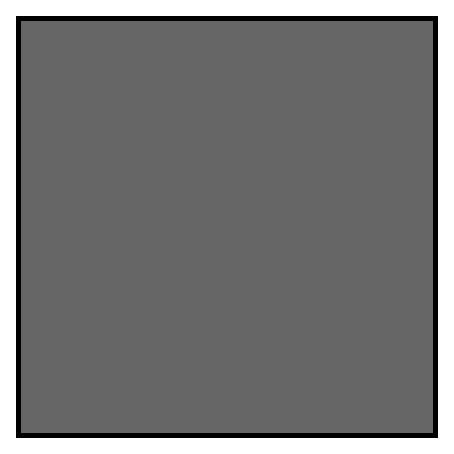
\includegraphics{example.eps}
% figure caption is below the figure
% \caption{Please write your figure caption here}
% \label{fig:1}       % Give a unique label
% \end{figure}
%
% For two-column wide figures use
% \begin{figure*}
% Use the relevant command to insert your figure file.
% For example, with the graphicx package use
  % 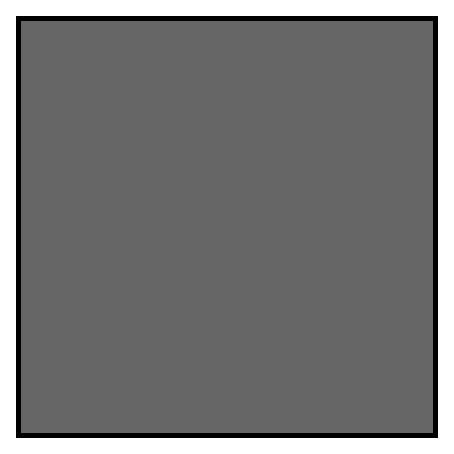
\includegraphics[width=0.75\textwidth]{example.eps}
% figure caption is below the figure
% \caption{Please write your figure caption here}
% \label{fig:2}       % Give a unique label
% \end{figure*}
%
% For tables use
% \begin{table}
% % table caption is above the table
% \caption{Please write your table caption here}
% \label{tab:1}       % Give a unique label
% % For LaTeX tables use
% \begin{tabular}{lll}
% \hline\noalign{\smallskip}
% first & second & third  \\
% \noalign{\smallskip}\hline\noalign{\smallskip}
% number & number & number \\
% number & number & number \\
% \noalign{\smallskip}\hline
% \end{tabular}
% \end{table}


%\begin{acknowledgements}
%If you'd like to thank anyone, place your comments here
%and remove the percent signs.
%\end{acknowledgements}


% Authors must disclose all relationships or interests that 
% could have direct or potential influence or impart bias on 
% the work: 
%
% \section*{Conflict of interest}
%
% The authors declare that they have no conflict of interest.


% BibTeX users please use one of
%\bibliographystyle{spbasic}      % basic style, author-year citations
%\bibliographystyle{spmpsci}      % mathematics and physical sciences
%\bibliographystyle{spphys}       % APS-like style for physics
%\bibliography{}   % name your BibTeX data base

% Non-BibTeX users please use
\begin{thebibliography}{}
%
% and use \bibitem to create references. Consult the Instructions
% for authors for reference list style.
%
\bibitem{RefJ}
% Format for Journal Reference
Author, Article title, Journal, Volume, page numbers (year)
% Format for books
\bibitem{RefB}
Author, Book title, page numbers. Publisher, place (year)
% etc
\end{thebibliography}

\end{document}
% end of file template.tex

